\subsection{TOPOLOGY OF A UNIFORM SPACE}

PROPOSITION 1. Let X be a set endowed with a uniform structure U, and for each \(x \in X\) let \(\mathfrak{B}(x)\) be the set of subsets \(\mathbf{V}(x)\) of \(\mathbf{X}(*)\) , where V runs through the set of entourages of U. Then there is a unique topology on X such that, for each \(x \in X\) , \(\mathfrak{B}(x)\) is the neighbourhood filter of x in this topology.

We have to show that the \(\mathfrak{B}(x)\) satisfy conditions \((\mathbf{V}_{\mathbf{I}})\) , \((\mathbf{V}_{\mathbf{II}})\) , \((\mathbf{V}_{\mathbf{III}})\) and \((\mathbf{V}_{\mathbf{IV}})\) of Chapter I, § 1, no. 2. That this is so for the first three of these conditions follows immediately from the fact that the entourages of \(\mathcal{U}\) satisfy \((\mathbf{F}_{\mathbf{I}})\) , \((\mathbf{F}_{\mathbf{II}})\) and \((\mathbf{U}_{\mathbf{I}})\) . As to \((\mathbf{V}_{\mathbf{IV}})\) , let \(\mathbf{V}\) be an entourage of \(\mathcal{U}\) , \(\mathbf{W}\) an entourage of \(\mathcal{U}\) such that \(\hat{\mathbf{W}} \subset \mathbf{V}\) ; then if \((x, y) \in \mathbf{W}\) and \((y, z) \in \mathbf{W}\) we have \((x, z) \in \mathbf{V}\) , so that \(\mathbf{W}(y) \subset \mathbf{V}(x)\) for all \(y \in \mathbf{W}(x)\) , and therefore \(\mathbf{V}(x) \in \mathfrak{B}(y)\) for all \(y \in \mathbf{W}(x)\) . This completes the proof.

DEFINITION 3. The topology defined in Proposition 1 is called the topology induced by the uniform structure U.

Examples. * 1) The topology induced by the additive uniformity on the set of real numbers is the topology of the real line (Chapter I, § 1, no. 2); similarly the topology induced by the additive uniformity on the set of rational numbers is the topology of the rational line. *

\begin{enumerate}
\def\labelenumi{\arabic{enumi})}
\setcounter{enumi}{1}
\tightlist
\item
  On any set X, the topology induced by the discrete uniformity (no. 1, Example 2) is the discrete topology.
\end{enumerate}

In the future, when we speak of the topology of a uniform space X, we shall always mean the topology induced by the uniform structure of the space, unless the contrary is expressly stated. The topological space obtained by putting this topology on the set X is sometimes called the topological space underlying the uniform space in question. For example, when we say that a uniform space is Hausdorff, or compact, or locally compact, etc., we mean that the underlying topological space has this property.

If X and \(X'\) are two uniform spaces, any isomorphism f of the uniform structure of X onto that of \(X'\) is also a homeomorphism of X onto \(X'\) ; we say that X is an isomorphism of the uniform space X onto the uniform space \(X'\) . It should be noted that a homeomorphism of X onto \(X'\) is not necessarily an isomorphism of the uniform structure of X onto that of \(X'\) .

\pandocbounded{
\includegraphics[keepaspectratio]{images/part001_037a61a5.jpg}}

In other words, distinct uniformities on the same set X can induce the same topology. * For example, on {]}0, +∞{[}, the additive and the multiplicative uniformities (which are distinct : Chapter III, § 6, Exercise 17) induce the same topology. *

For another example see § 2, no. 2, Remark 1.

PROPOSITION 2. Let X be a uniform space. For every symmetric entourage V of X and every subset M of X × X, VMV is a neighbourhood of M in the product space X × X, and the closure of M in this space is given by the formula

\[
\overline {{\mathbf {M}}} = \bigcap_ {\mathbf {V} \in \mathfrak {S}} \mathbf {V M V}\tag{I}
\]

where \(\mathfrak{S}\) denotes the set of symmetric entourages of \(\mathbf{X}\) .

Let V be a symmetric entourage of X. The relation \((x, y) \in \text{VMV}\) means that there is an element \((p, q)\) of M such that \((x, p) \in V\) and \((q, y) \in V\) : in other words (V being symmetric) \(x \in V(p)\) and \(y \in V(q)\) , that is \((x, y) \in V(p) \times V(q)\) . Since \(V(p) \times X(q)\) is a neighbourhood of \((p, q)\) in \(X \times X\) , the first part of the proposition is proved. The relations \((x, p) \in V\) , \((y, q) \in V\) can also be written \(p \in V(x)\) , \(q \in V(y)\) or \((p, q) \in V(x) \times V(y)\) . As V runs through S, the sets \(V(x) \times V(y)\) form a fundamental system of neighbourhoods of \((x, y)\) in \(X \times X\) ; for if U, \(U'\) are any two entourages there is always a symmetric entourage \(V \subset U \cap U'\) , so that \(V(x) \times V(y) \subset U(x) \times U'(y)\) . Hence \(V(x) \times V(y)\) meets M for each \(V \in S\) if and only if \((x, y) \in \overline{\mathbf{M}}\) , and formula (1) follows.

COROLLARY 1. If A is any subset of X and V is any symmetric entourage of X, then V(A) is a neighbourhood of A in X, and

\[
\overline {{{\mathbf {A}}}} = \bigcap_ {\mathbf {v} \in \mathfrak {S}} \mathbf {V} (\mathbf {A}) = \bigcap_ {\mathbf {v} \in \mathfrak {U}} \mathbf {V} (\mathbf {A})\tag{2}
\]

where \(\mathfrak{U}\) denotes the set of all entourages in \(\mathbf{X}\) .

If \(\mathbf{M} = \mathbf{A} \times \mathbf{A}\) , then \(\mathrm{VMV} = \mathrm{V}(\mathbf{A}) \times \mathrm{V}(\mathbf{A})\) for any \(\mathbf{V} \in \mathfrak{S}\) ; for the relation ``there exists \(p \in \mathbf{A}\) such that \((x, p) \in \mathbf{V}"\) is by definition equivalent to \(x \in \mathbf{V}(\mathbf{A})\) . The corollary now follows from Chapter I, § 4, no. 2, Proposition 5 and no. 3, Proposition 7.

V(A) is said to be the V-neighbourhood of A.

If V is an entourage which is open in X × X, then V(x) is open in X for each x ∈ X (Chapter I, § 4, no. 2, Corollary to Proposition 4) and therefore V(A), being the union of the V(x) as x runs through A, is open in X. On the other hand, if V is a closed entourage in X × X, V(A) need not be closed in X for every subset A of X (Exercise 3).

\pandocbounded{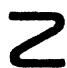
\includegraphics[keepaspectratio]{images/part001_f8cd4ad5.jpg}}

It should also be remarked that as V runs through the set of entourages of X, the sets V(A) do not necessarily form a fundamental system of neighbourhoods of A in X (Exercise 2).

COROLLARY 2. The interiors (resp. the closures) of the entourages of X in X × X form a fundamental system of entourages of X.

If V is any entourage of X, there is a symmetric entourage W such that \(W \subset V\) ; since W is a neighbourhood of W (Proposition 2), the interior of V in \(X \times X\) contains W and is therefore an entourage. Furthermore, we have \(W \subset W \subset W \subset V\) by Proposition 2, and hence V contains the closure of an entourage.

COROLLARY 3. Every uniform space satisfies axiom (O \(_{III}\) ).

If \(x\) is any point of \(X\) and \(V\) runs through the entourages of \(X\) which are closed in \(X \times X\) , then the sets \(V(x)\) form a fundamental system of neighbourhoods of \(x\) in \(X\) by Corollary 2, and they are closed in \(X\) (Chapter I, § 4, no. 2, Corollary to Proposition 4).

PROPOSITION 3. A uniform space X is Hausdorff if and only if the intersection of all the entourages of its uniform structure is the diagonal \(\Delta\) of \(X \times X\) . Every Hausdorff uniform space is regular.

The latter statement follows immediately from Corollary 3 to Proposition 2. We have seen that the closed entourages form a fundamental system of entourages (Proposition 2, Corollary 2); if their intersection is \(\Delta\) , then \(\Delta\) is closed in \(X \times X\) and consequently \(X\) is Hausdorff (Chapter I, § 8, no. 1, Proposition 1). Conversely, if \(X\) is Hausdorff then for every point \((x, y) \notin \Delta\) there is an entourage \(V\) of \(X\) such that \(y \notin V(x)\) , or equivalently \((x, y) \notin V\) ; hence \(\Delta\) is the intersection of all the entourages.

If a uniform space X is Hausdorff, we say that the uniform structure of X is Hausdorff. If B is a fundamental system of entourages for this structure; then X is Hausdorff if and only if the intersection of all the sets of B is \(\Delta\) .

